\documentclass[12pt]{article}
\usepackage[margin=2cm]{geometry} 
\usepackage{titling}
\usepackage{graphicx}
\usepackage{float}
\usepackage[hidelinks]{hyperref}
\usepackage[italian]{babel}
\usepackage{subcaption}

\setlength\parindent{0pt}
\setlength{\parskip}{1em}
\setlength{\droptitle}{-2cm}

\title{Istruzioni d'uso Ping Pong 3D (ad uso interno)}
\author{Università della Svizzera italiana}
\date{Versione \today}


\begin{document}
\maketitle
\tableofcontents
\newpage


\section{Installazione}\label{installation}	

	\subsection{Componenti}
	
		\begin{itemize}
			\item computer
			\item Kinect v2
			\item supporto Kinect (3 pezzi)
			\item proiettore 3D
			\item sync box 3D EXXR
			\item occhiali 3D attivi
			\item racchetta gialla
			\item 2 cavi DVI-I lunghi
			\item 2 cavi alimentazione
			\item cavo 3D box (coax - VESA)
			\item cavo alimentazione 3D box (24V)
		\end{itemize}
		
		
	\subsection{Montaggio}
	
		\begin{enumerate}
			\item Collegare l'alimentazione e i due cavi DVI al proiettore
			\item Collegare l'alimentazione e i due cavi DVI al PC
			\item Collegare l'alimentazione del Kinect e il cavo USB (blu) ad una porta USB 3.0 (blu) del PC
			\item Collegare la sync box all'alimentazione e al proiettore (\texttt{External sync})
		\end{enumerate}

		\begin{figure}[H]
			\centering
			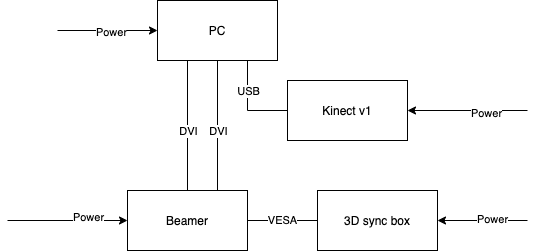
\includegraphics[width=0.9\textwidth]{img/cablesScheme.png}
			\caption*{Lo schema di collegamento dei cavi}
		\end{figure}
		
		\begin{figure}[H]
			\centering
			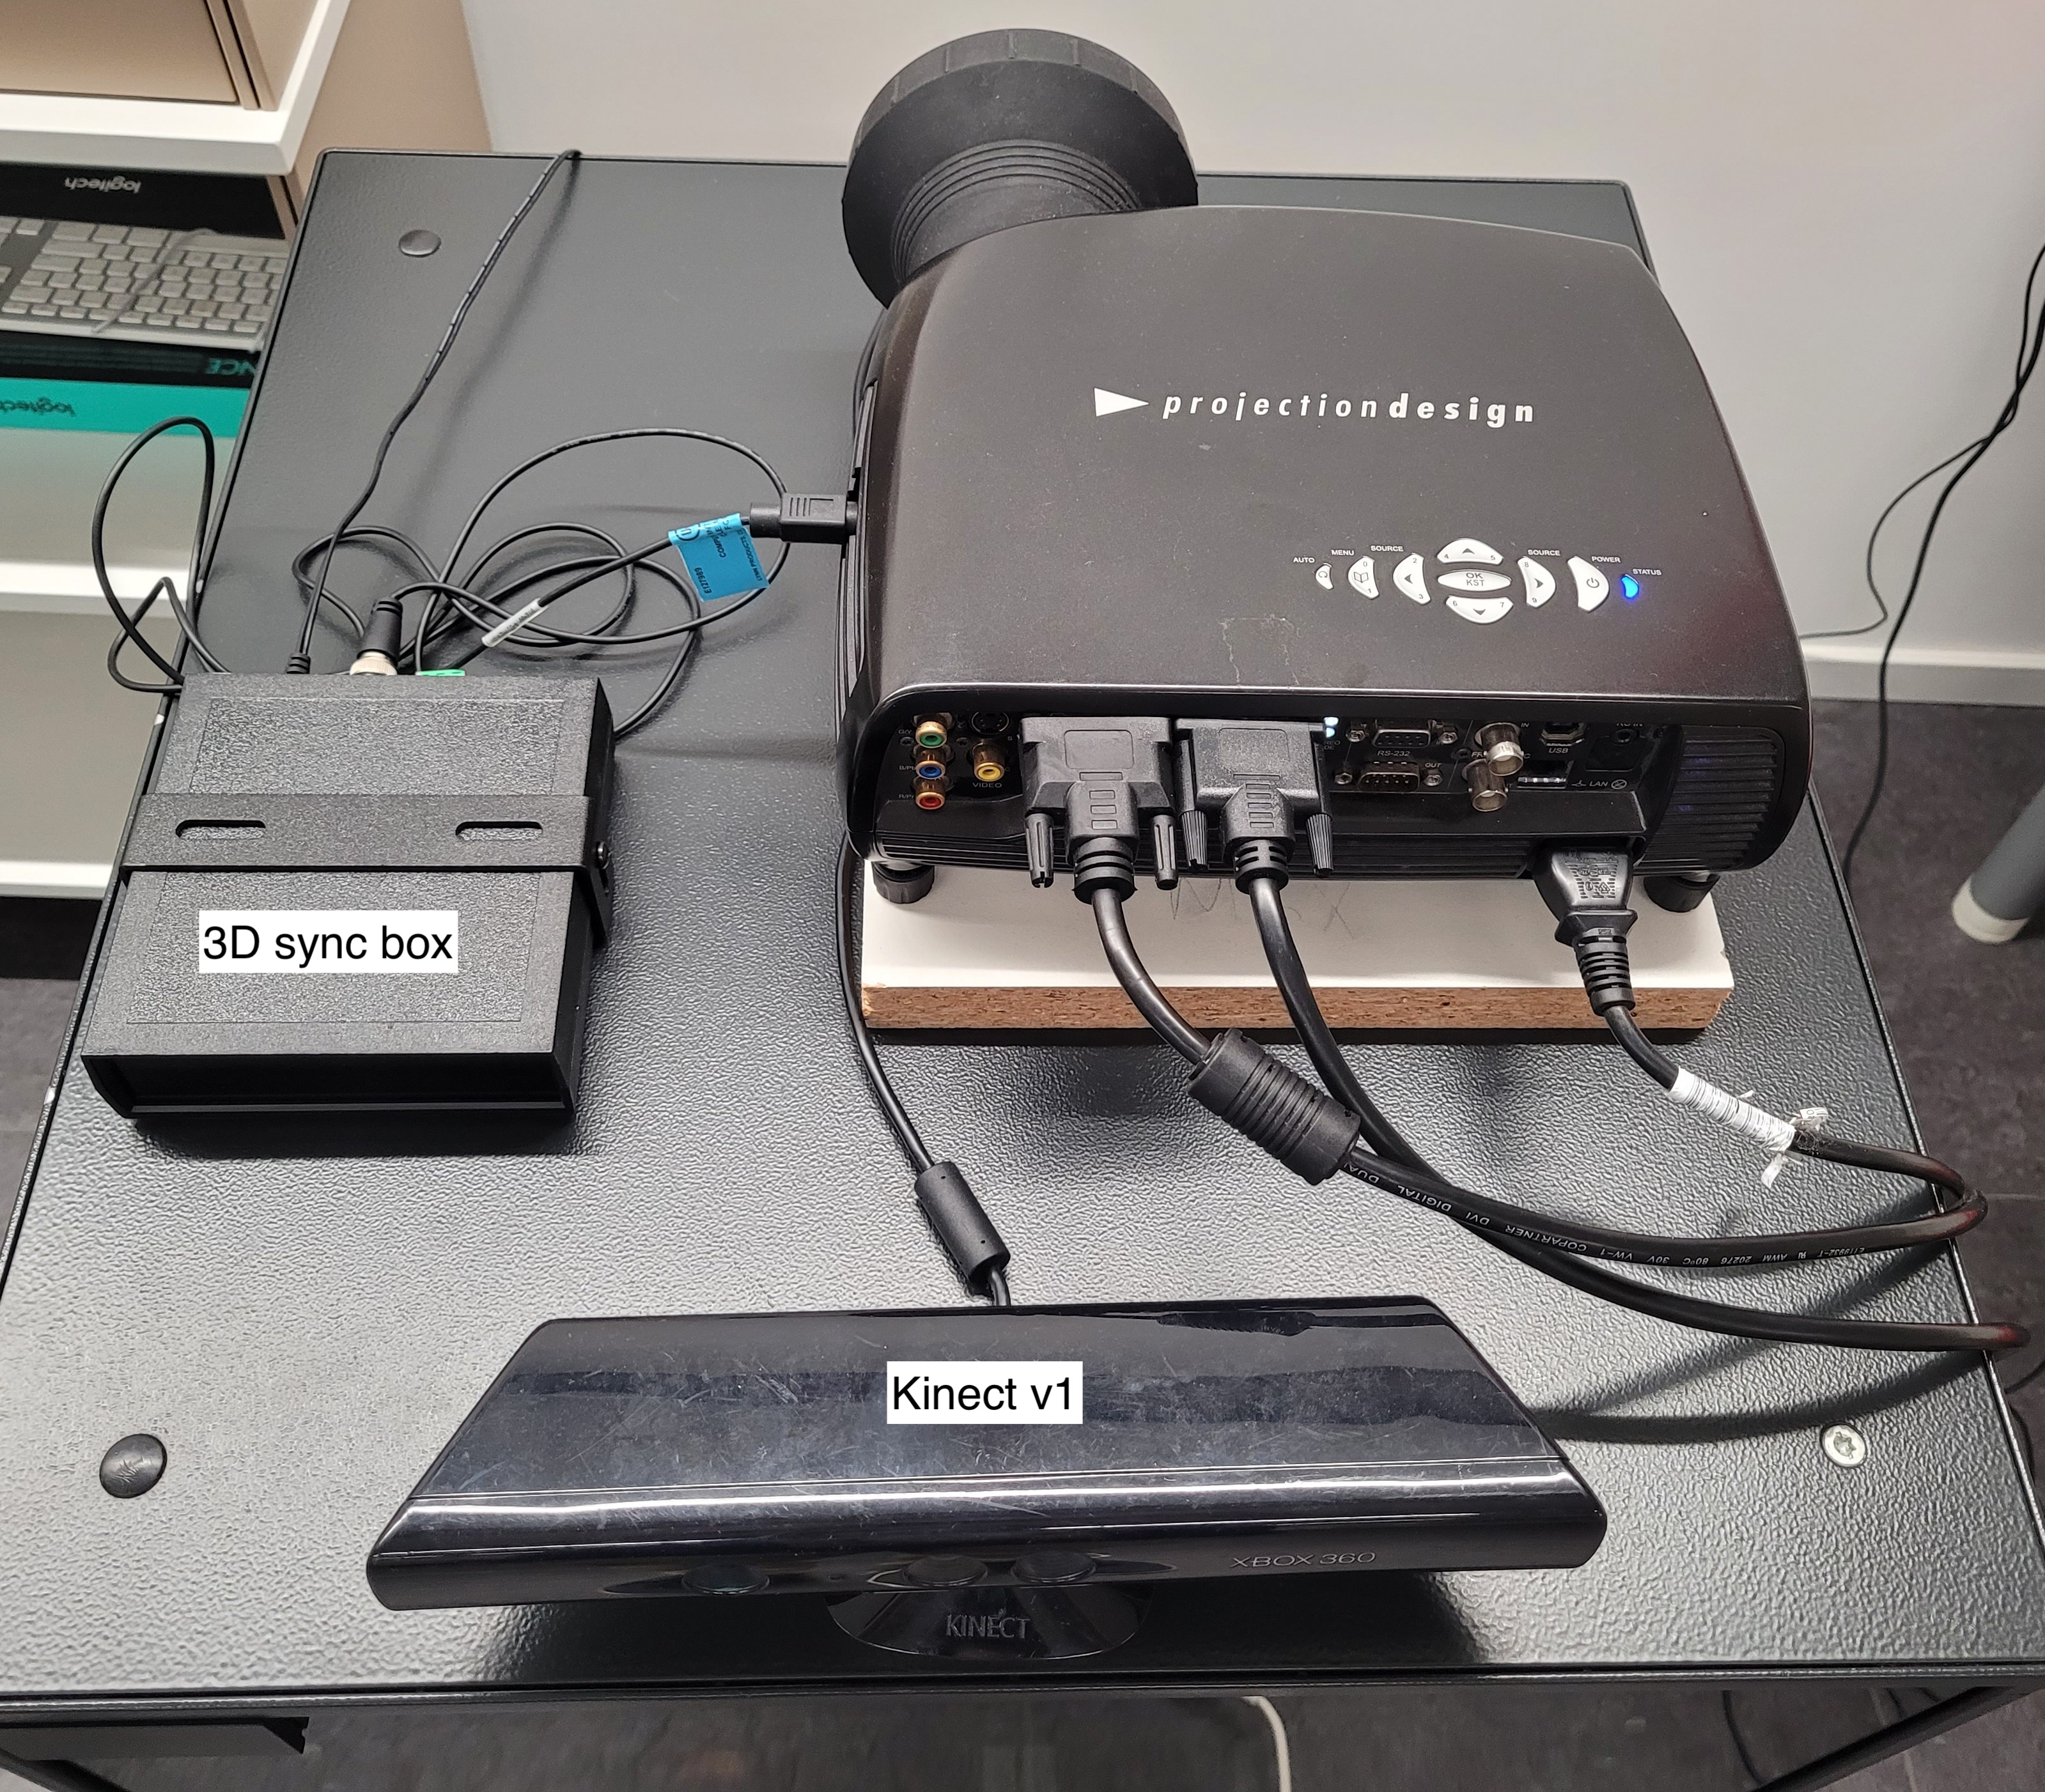
\includegraphics[width=0.9\textwidth]{img/beamer.jpg}
			\caption*{Il materiale assemblato}
		\end{figure}
		
		
	\newpage
	\subsection{Avvio}

		Accendere il proiettore, dopodiché avviare il PC e cliccare sul collegamento
		\texttt{tableTennis} sul Desktop. Controllare che il proiettore sia in modalità 3D
		(menu $\rightarrow$ stereo $\rightarrow$ stereo mode).

		Se l'immagine non dovesse essere in 3D, controllare i parametri del pannello di controllo Nvidia
		come segue: 

		\begin{figure}[H]
			\centering
			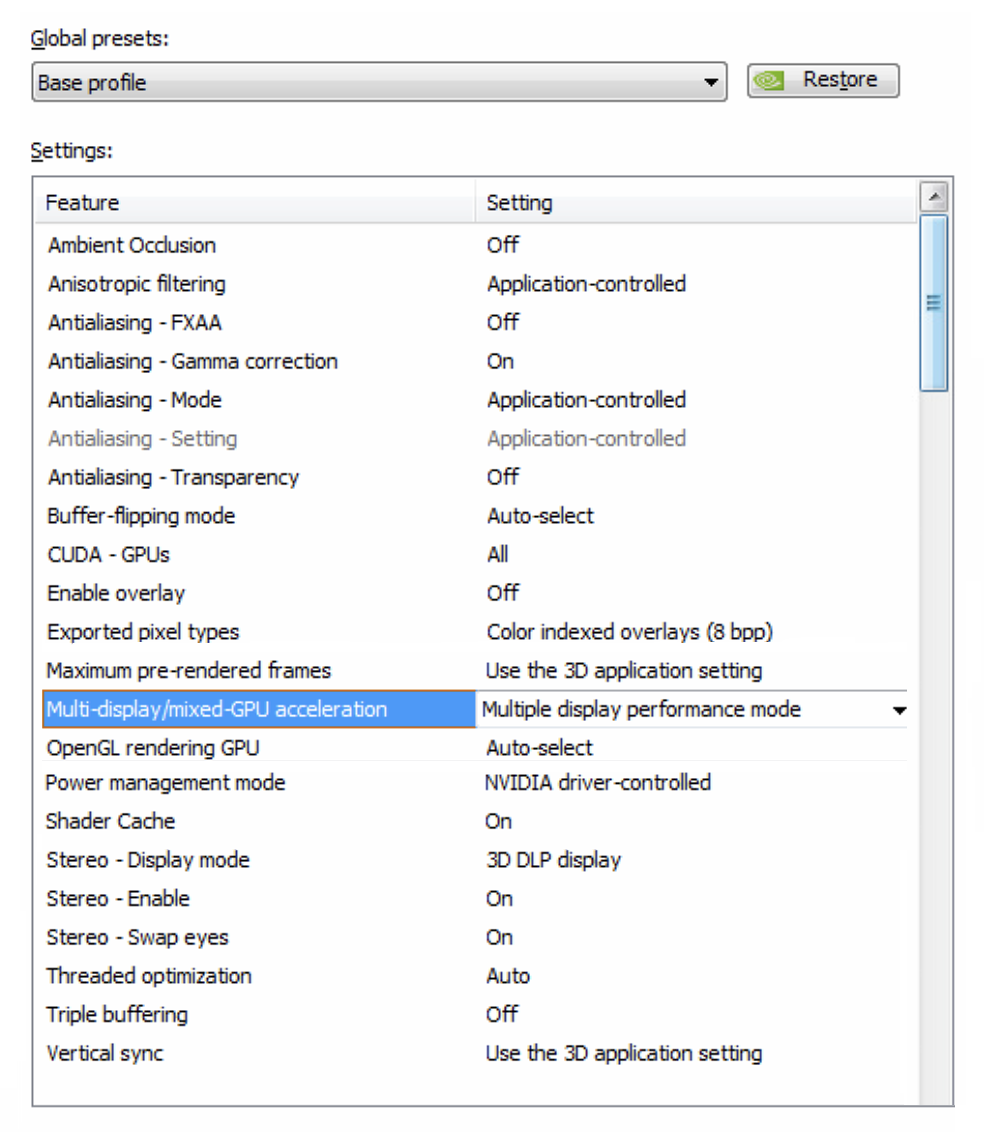
\includegraphics[width=0.9\textwidth]{img/params.png}
			\caption*{I parametri corretti per il software 3D}
		\end{figure}

	\subsection{Spegnimento}
	
	Premere ESC per uscire dal programma, dopodiché arrestare normalmente il sistema e 
	premere due volte il tasto \texttt{Power} del beamer per spegnerlo. \textbf{NON} scollegarlo finché
	il LED arancione lampeggia (raffreddamento in corso)!
		
		
\section{Utilizzo}

	\subsection{Tasti utili}
	
	\begin{tabular}{l l}
		ESC & esci\\
		A/Y & aumenta/riduci raggio scena\\
		M & torna al menù\\
		K & gioca\\
		L & replay\\
		Sinistra/Destra & aumenta/riduci angolo\\
		Su/Giù & aumenta/riduci distanza\\
	\end{tabular}
		
		
\section{Codice sorgente}

	Il codice sorgente dell'applicazione, assieme alle istruzioni per compilarla, si trova alla pagina \url{https://github.com/USI-Showroom/3DTableTennis}.
		
	
\end{document}
